\documentclass[12pt,twoside]{article}

% Language setting
% Replace `english' with e.g. `spanish' to change the document language
\usepackage[english]{babel}

% Set page size and margins
% Replace `letterpaper' with `a4paper' for UK/EU standard size
\usepackage[letterpaper,top=2cm,bottom=2cm,left=3cm,right=3cm,marginparwidth=1.75cm]{geometry}

% Useful packages
\usepackage{mathptmx} %% For TImes New Roman Font
\usepackage{amsmath}
\usepackage{graphicx}
\usepackage[colorlinks=true, allcolors=blue]{hyperref}
%\usepackage{fancyhdr}

\title{Title: Preventive Maintenance of Industrial Rotational Machinery through Machine Learning and Acoustic Monitoring}
\author{Design Contest, VLSID 2025, Bengaluru}

\begin{document}
\maketitle

\begin{abstract}
High-performance rotational machinery is crucial for numerous industrial fields, such as rolling mills, turbines, and raw material processing. To maintain dependable operation, early fault detection is important and should minimize maintenance and repair expenses. We propose an acoustic monitoring system that will use machine learning to detect faults in an early stage to avoid costly maintenance and repair. This method provides an efficient and affordable means to monitor the condition of industrial equipment and prevent failures. 
The implementation of digital signal processing (DSP) and machine learning (ML) will be conducted on the Texas Instruments' SK-AM62A-LP AI accelerator evaluation board (EVM). The EVM will be interfaced with a microphone that will pick up the acoustic vibrations from the rotational machines and detect early faults, leading to considerable cost reductions for stakeholders with minimal expenditure.
\end{abstract}

%%%--- HARDWARE PLATFORM
\section{Hardware Platform}

\subsubsection*{Texas Instruments’ SK-AM62A-LP}

%%%---FIGURE: TI Board
%%\begin{figure}[htb]
%\centering
%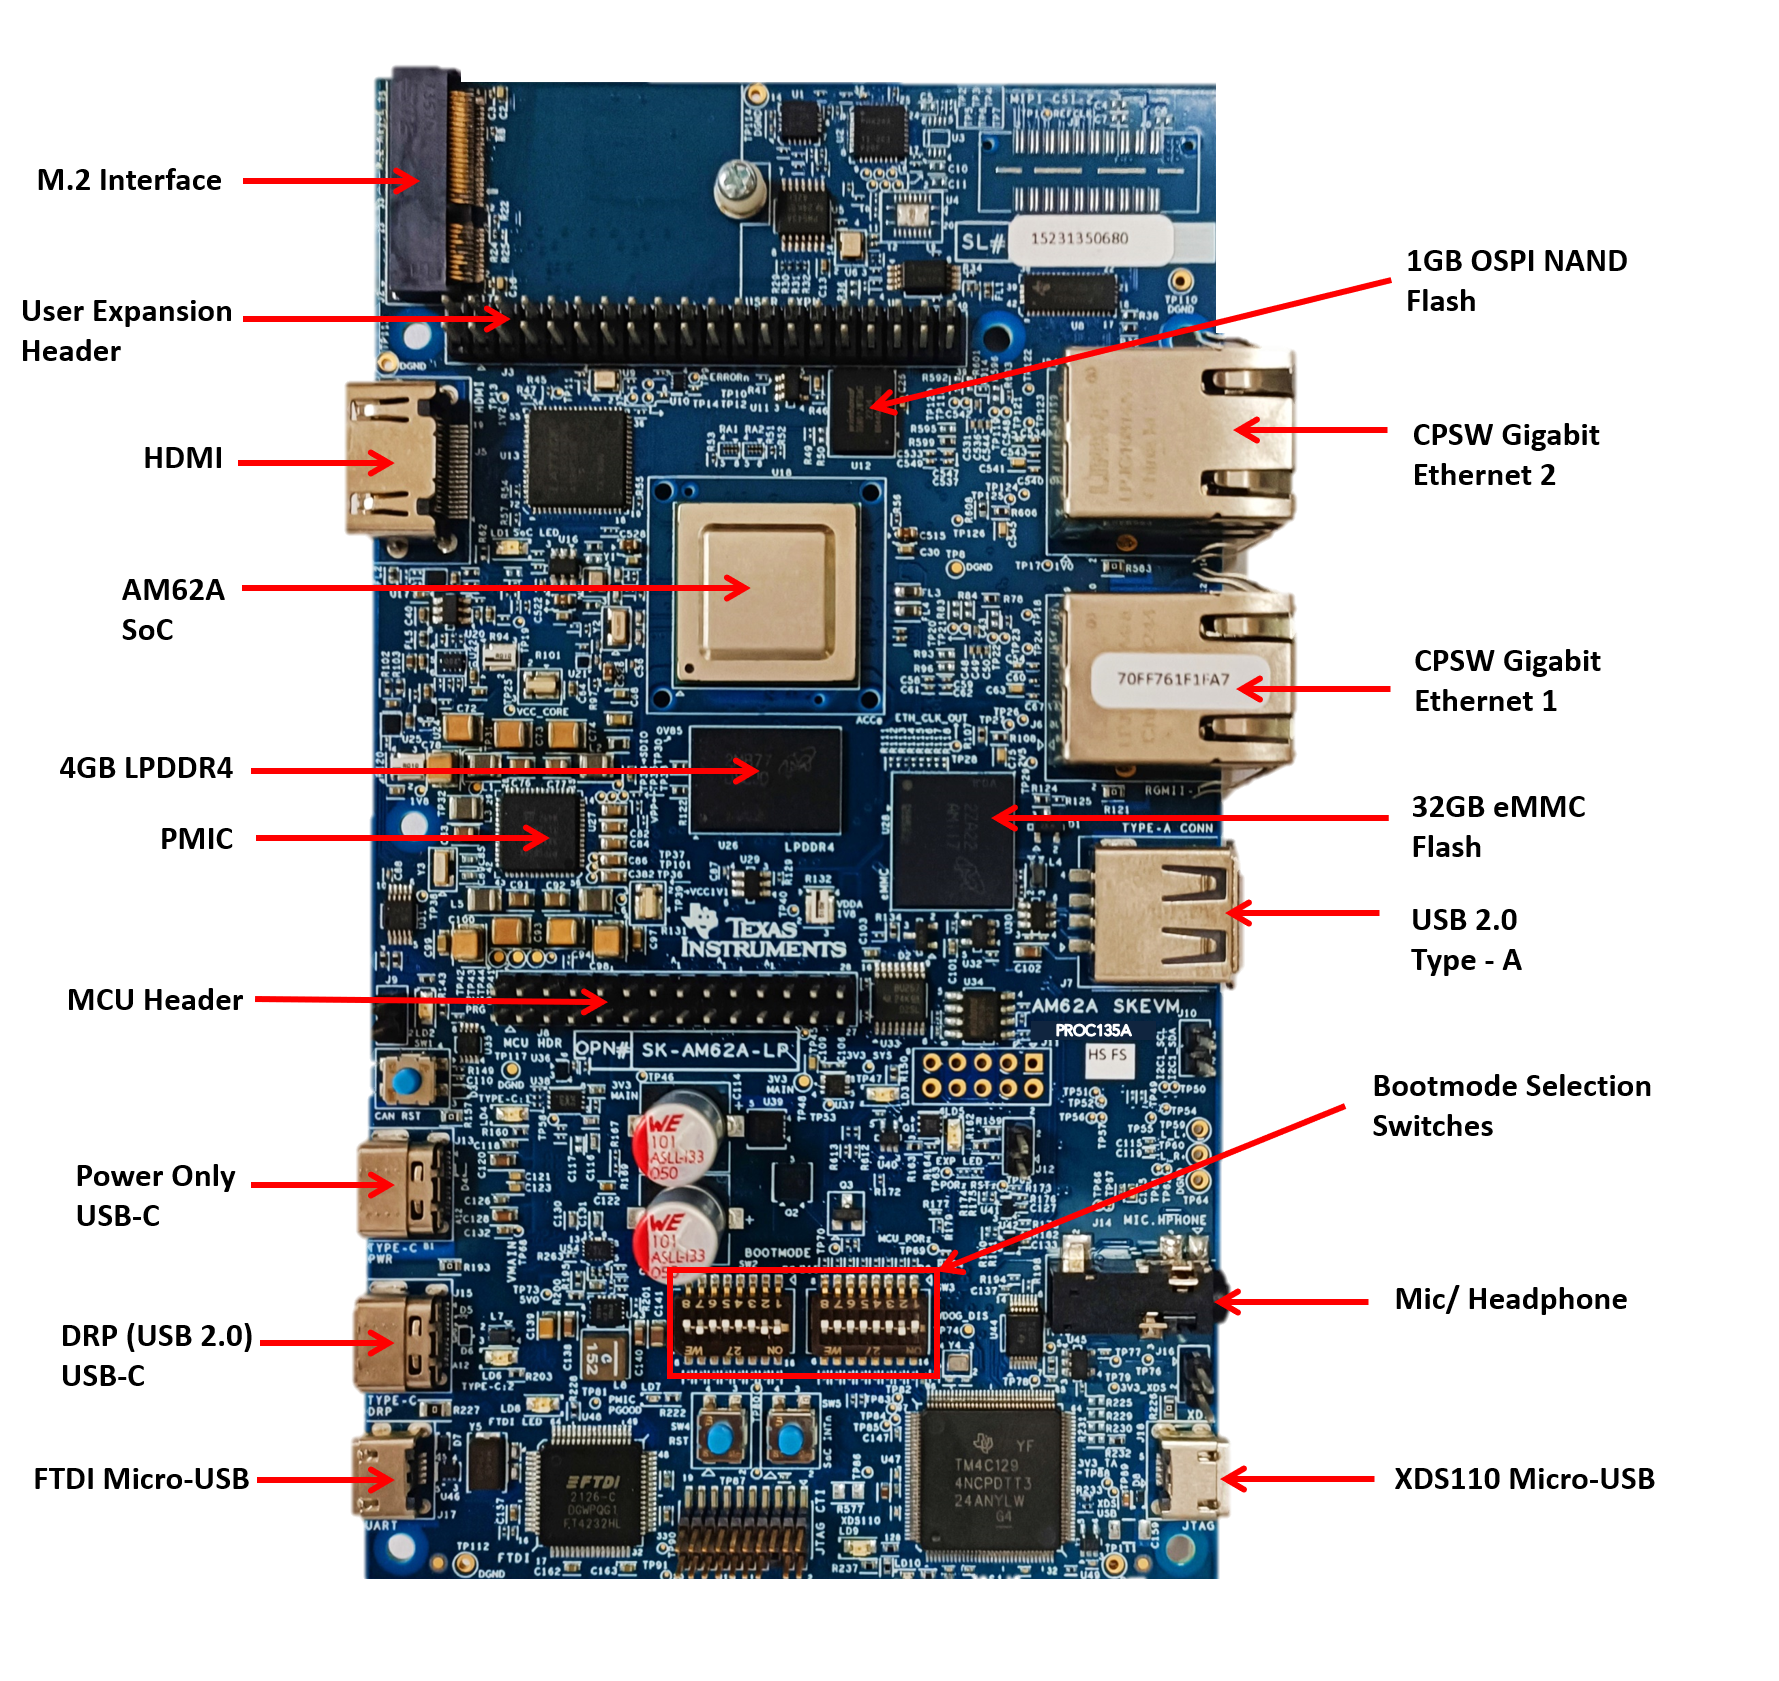
\includegraphics[width=0.45\linewidth]{figs/TI-devBrd-RE3.png}
%\caption{\label{fig:TIbrd}TI Development board.}
%\end{figure}

\href{https://www.ti.com/tool/SK-AM62A-LP}{Texas Instruments' SK-AM62A-LP} starter kit is designed for developers working with low-power Sitara\textsuperscript{TM} processors, particularly the AM62A AI vision processor with a quad-core 64-bit Arm Cortex-A53 with access to 4GB LPDDR4.
It has 2 TOPS AI accelerator and an image signal processor (ISP) supporting up to 5 MP at 60 fps supporting H.264/H.265 video encoding/decoding. 
It has a wide range of ports including the MIPI CSI-2 camera interface, HDMI output with audio codec support, USB Type-A 2.0, USB Type-C dual-role device (supports USB booting), onboard JTAG emulator, and UARTs via USB Type-B.
It has bootable interfaces including removable microSD, USB, QSPI, Ethernet, and UART.

For software support, it supports \textit{TI Processor SDK Linux} OS and \textbf{RT-Linux} for real-time applications. The development tools are compatible with \textit{Code Composer Studio\textsuperscript{TM}} IDE for debugging and emulation.

%%%--- EXPLANATION OF IDEA
\section{Explanation of the Idea}
% Include a block diagram, overview of implementation  (Minimum font size: 10pt, Times New Roman font. Maximum two pages including tables, diagram, references (if any) )

High-performance rotational machinery is crucial to numerous industrial fields such as rolling mills, turbines, and raw material processing.
A recent study of more than 400 malfunctioning of just one type of pumps, multistage centrifugal pumps (MCPs), found that the industry suffered more than 6000 hours of maintenance-related downtime due to the absence of precise and intelligent fault diagnosis (FD), incurring a cost in the range of 50 million USD \cite{rane2021re}.
The vast array of uses for rotational machinery implies that malfunctions can have major repercussions, such as energy waste, industrial process interruptions, financial losses, costly repairs, and jeopardized employee safety. 

To maintain dependable operation, early fault detection is important and should minimize maintenance and repair expenses. Consistent supervision can be achieved using affordable and reliable signal processing and artificial intelligence (AI) techniques \cite{sunal2022review}. Artificial intelligence techniques for fault detection involve preprocessing signals and features to identify and classify faults \cite{saeed2021fault, jiang2019bearing}.

%%%---FIGURE: Architecture
\begin{figure}[htb]
\centering
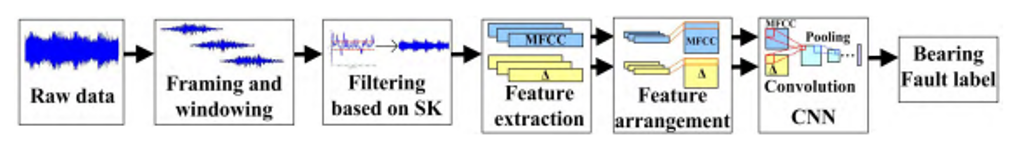
\includegraphics[width=1.0\linewidth]{figs/fig-arch1.png}
\caption{\label{fig:arch1}Proposed architecture of the fault detection using audio analytics and machine learning.}
\end{figure}

The proposed architecture of the fault detection system is shown in Figure~\ref{fig:arch1}. This design closely resembles the detection of voice keywords, commonly known as keyword spotting (KWS), a technique that has been used effectively for many years \cite{chong20220}.
In this architecture, \textit{digitized} microphone signal is passed through digital signal processing steps to extract some spectral features of the audio signal known as mel-frequency cepstral coefficients (MFCC). These coeeficients are used to train a neural network such as Convolutional neural network (CNN) or Recurrent neural network (RNN). 

Digital audio data are first high-pass filtered, typically performed by $y[n] = x[n] - \alpha~x[n-1]$ where $\alpha$ typically ranges from 0.9 to 1 \cite{han2006efficient}.
Next, a window function (e.g., Hanning) is applied to the data to minimize spectral leakage during the fast Fourier transform (FFT) process. The linear spectrum is transformed into a Mel scale for better computing efficiency using the following equation $Mel(f) = 2595\cdot \log(1 + f/700)$ \cite{han2006efficient}.
Subsequently, the logarithm of the Mel frequency power is computed followed by the discrete cosine transform (DCT) to generate the MFCC coefficients. These coefficients are then fed into a \textit{trained} classifier (CNN/RNN) to detect and report faults.

%%%---FIGURE: TI-EVM-Setup
\begin{figure}[htb]
\centering
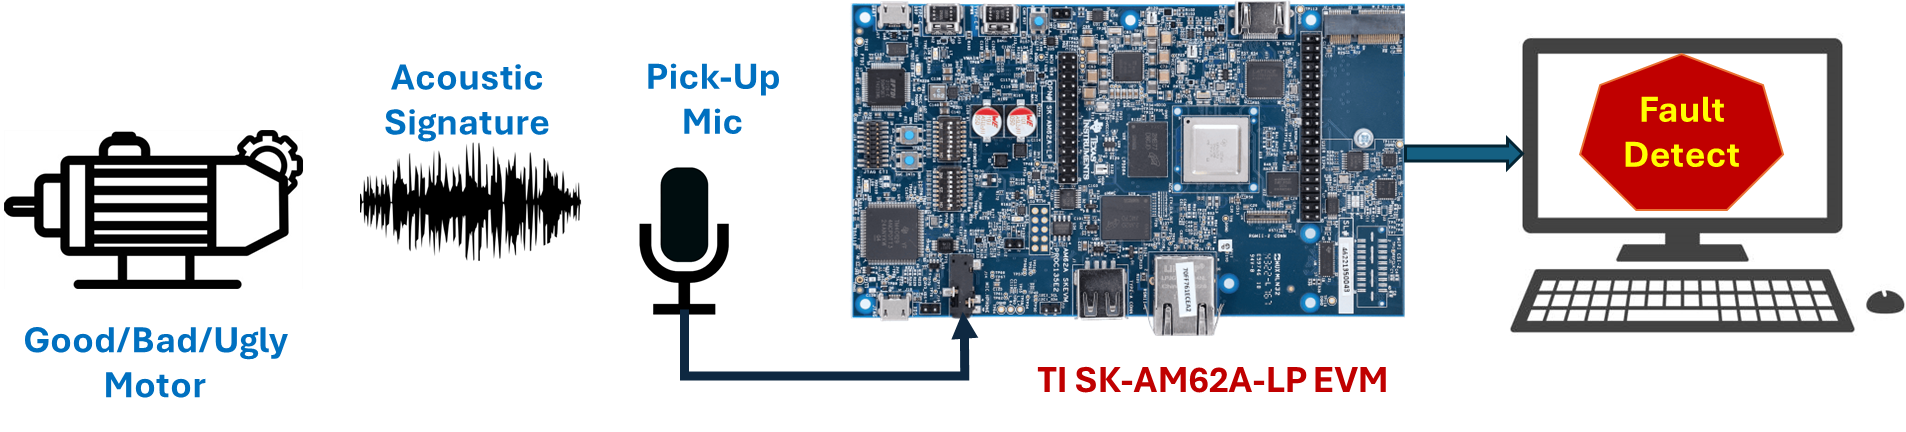
\includegraphics[width=1.0\linewidth]{figs/TI-EVM-Setup.png}
\caption{\label{fig:TI-EVM-setup}Real-time setup with the TI SK-AM62A-LP EVM to monitor fault in motor bearing systems.}
\end{figure}

Figure~\ref{fig:TI-EVM-setup} illustrates the real-time configuration of the proposed fault detection system. An analog microphone captures the audio signal from motor vibrations, which is connected to the EVM board through the 3.5mm microphone jack. The internal audio codec (TLV320AIC3106I RGZT) converts the analog signal into a serial $I2C$ digital stream. The digital data is subsequently processed and categorized as depicted in Figure~\ref{fig:arch1} and described afterward. 

In the \textit{training phase}, the acoustic data from the \href{https://engineering.case.edu/bearingdatacenter}{Case Western Reserve University (CWRU) database}\cite{case2019} will be used directly rather than the microphone data. After training the neural network (CNN / RRN), the neural network \textit{weights} will be \textit{frozen} for real-time fault diagnosis.

To test and demonstrate the system, the CWRU bearing data will be played through a speaker, and a microphone will capture the audio signal to perform a real-time fault diagnosis, as illustrated in Figure~\ref{fig:TI-EVM-setup}.


\section{Example of its Application}
% application (Describe an example consisting of potential application/Future application. This will enable usage model towards its market acceptance) (maximum 200 words)
Rotating equipment like motors, pumps, fans and compressors are prime candidates for acoustic monitoring \cite{judith2017}. Acoustic sensors identify irregularities in the noise produced by rotating parts, facilitating the early detection of faults.

Acoustic sensors can also be used to detect faults in valves, pipelines, and other fluid systems \cite{judith2017}. Leaks, obstructions, and cavitation in valves emit distinct acoustic signals that can be identified. Acoustic monitoring is able to detect problems such as valve seat leaks, stuck valves, and piping erosion / corrosion before they develop into major problems.

Sound-based monitoring can also be used to assess the condition of electrical systems such as transformers, switchgear, and motors \cite{avinton2023}. Acoustic emissions generated by partial discharges, arcing, and the corona in an electrical apparatus can be detected using sound sensors. This facilitates the early detection of insulation wear, loose connections, and various electrical problems.

For this design contest, we will focus on rolling element bearings (REB), one of the most common components in rotating machines, and they are also one of the main reasons for failures \cite{jiang2019bearing}. 
Failures arise from heavy loads, poor lubrication, and foreign matter due to bad sealing. Effective fault classification methods are needed for safe operation. Sound analysis offers an excellent approach for the early identification of different bearing faults, leading to considerable cost reductions for stakeholders with minimal expenditure. \href{https://engineering.case.edu/bearingdatacenter}{Case Western Reserve University (CWRU) database} \cite{case2019} offers an extensive data set to train and develop the model shown in Figure~\ref{fig:arch1}. 

\section{Benefits and Value Addition}
% (Explain the key benefits of your idea/implementation. You should describe the key value addition of your idea as this will explain why your idea has value in the presence of other participants. It will show uniqueness/Unique selling point/key differentiator) (maximum 200 words)

Acoustic monitoring offers several notable advantages over conventional preventive maintenance methodologies, which include vibration analysis, parameter monitoring, and invasive techniques:
\begin{itemize}
    \item Ability to \textit{detect certain faults earlier} than traditional methods.
    \item \textit{Cost-effectiveness}, as acoustic sensors are less expensive than, e.g., vibration sensors.
    \item Implementing the system is straightforward because it operates at low frequencies, leading to \textit{inexpensive monitoring solutions}.
    \item \textit{Versatility} to monitor a wide range of equipment and systems.
    \item \textit{Non-invasive} monitoring as sensors can be placed remotely without contact with the machine.
\end{itemize}

In brief, acoustic surveillance serves as a robust method for predictive maintenance, leveraging AI and machine learning to scrutinize machine sounds and identify irregularities at an early stage. It provides an efficient and affordable means to supervise the condition of industrial equipment and avert failures.


\section{Team Members}
% •	List your team members’ names, program, department, year of study and contact emails here
\begin{table}[h]
    \centering
    \begin{tabular}{|c|c|c|c|c|}
        \hline
        \textbf{Name} & \textbf{Program} & \textbf{Dept.} & \textbf{Year} & \textbf{Email} \\ \hline\hline
        & & & & \\ \hline
        & & & & \\ \hline
        & & & & \\ \hline
        & & & & \\ \hline
    \end{tabular}
    \caption{Team Member Information}
    \label{tab:student_info}
\end{table}

\section{University Address}
% •	Include the name of your university/college and your institute’s postal address to ship the boards
Silicon University \\
Silicon Hills Road, Patia \\
Bhubaneswar, 751024, ODISHA

\section{Contact Person}
% •	Mention one contact person from the institute, his/her official/institute email id, and contact phone number.
Saroj Rout \\
Additional Professor, Electronics Engineering Department \\
Silicon University, Odisha \\
\textit{Email}: \texttt{saroj.rout@silicon.ac.in} \\
\textit{Phone}: +91-90907-52283 \\


\bibliographystyle{ieeetr}
\bibliography{reference}

\end{document}